\documentclass[a4paper ,12pt, onecolumn]{article}
\usepackage[utf8]{inputenc}
\usepackage[spanish]{babel}
\usepackage[hidelinks]{hyperref}
\usepackage{graphicx}
\begin{document}
\title{Anexo desarrollo de hardware}

\author{Rubén Arce}
\date{\today}
\maketitle
\cleardoublepage
\tableofcontents
\cleardoublepage

\section{Introducción}
\section{Emisor beacon}
    \subsection{Aspectos a considerar}
        \begin{enumerate}
            \item Bajo consumo
            \item Tamaño reducido
            \item bluetooth
        \end{enumerate}
    \subsection{Circuito eléctrico}
    \subsection{PCB de control}
    \subsection{Imágenes renderizado}   
        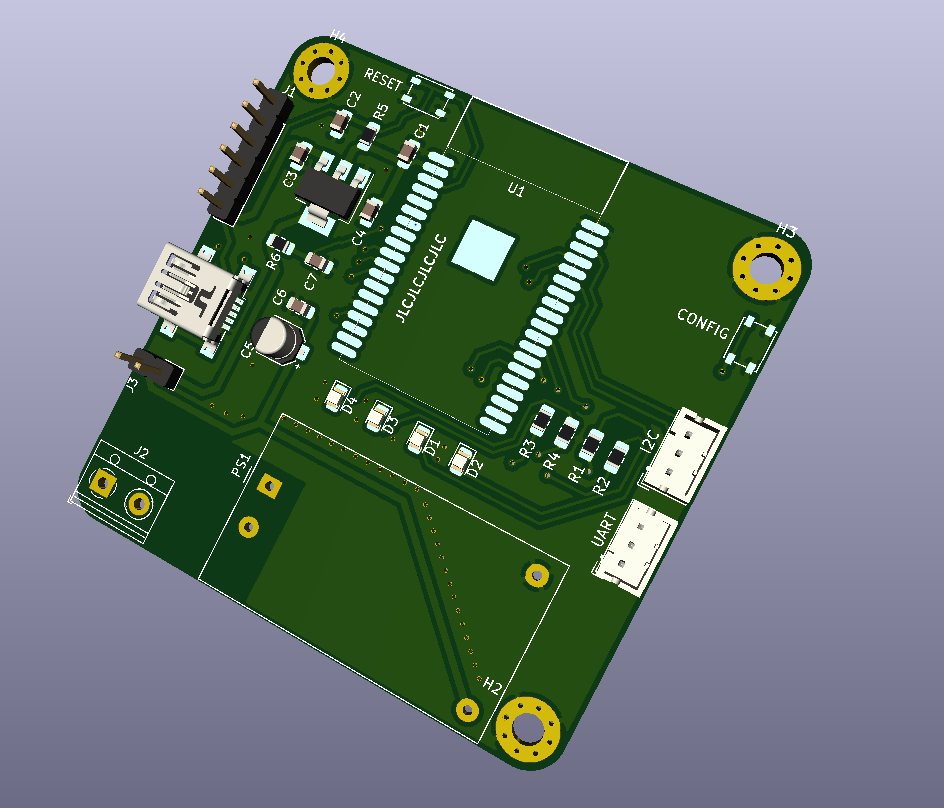
\includegraphics[scale=0.4]{../receiver_1.PNG}
        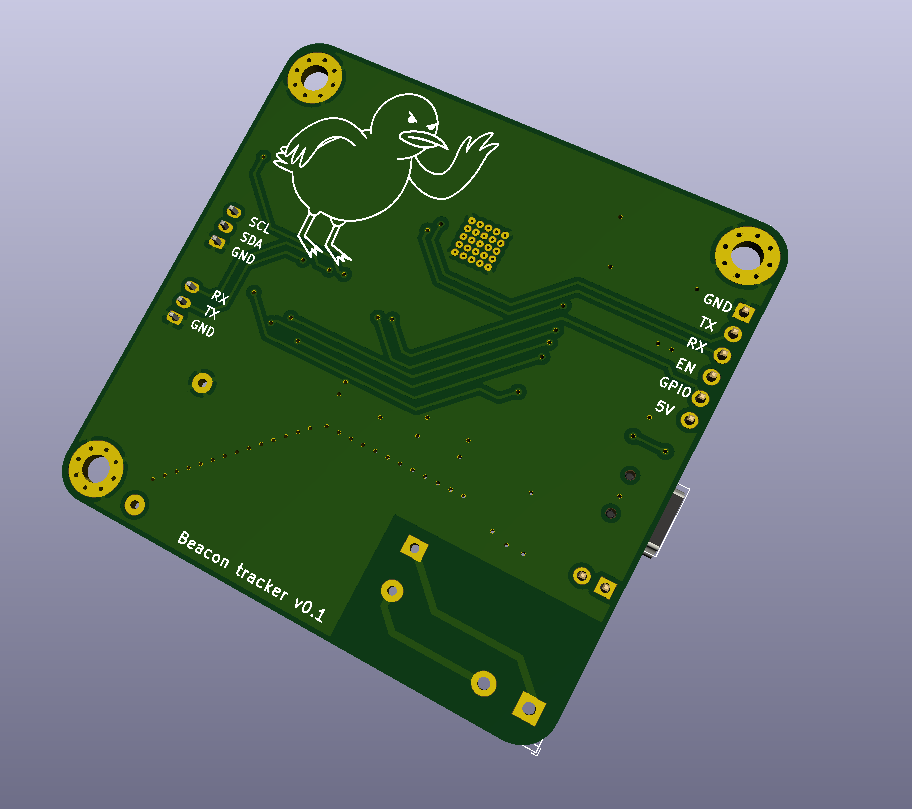
\includegraphics[scale=0.4]{../receiver_2.PNG}
    \subsection{Imágenes reales}

\section{Receptor beacon o gateway}
    \subsection{Aspectos a considerar}
        \begin{enumerate}
            \item Velocidad de procesamiento:
            \item Wifi/bluetooth:
        \end{enumerate}
    \subsection{Circuito eléctrico}
    \subsection{PCB de control}
    \subsection{Imágenes renderizado}
        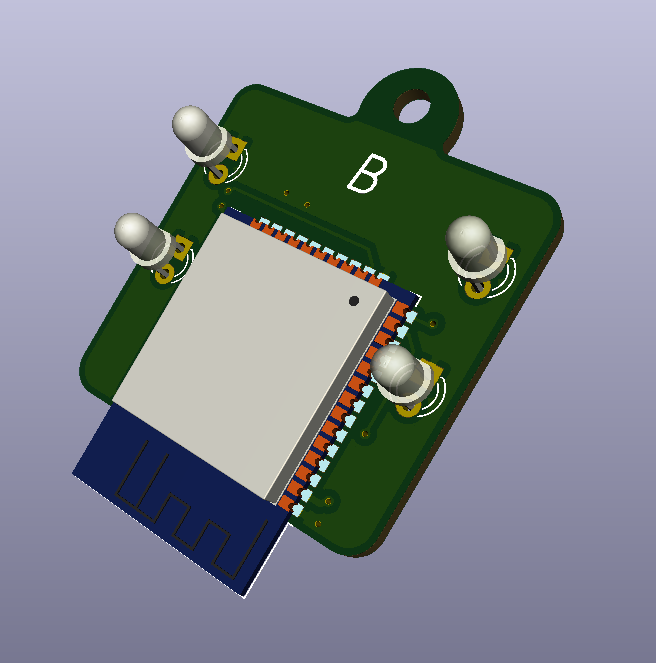
\includegraphics[scale=0.4]{../emiter_1.PNG}
        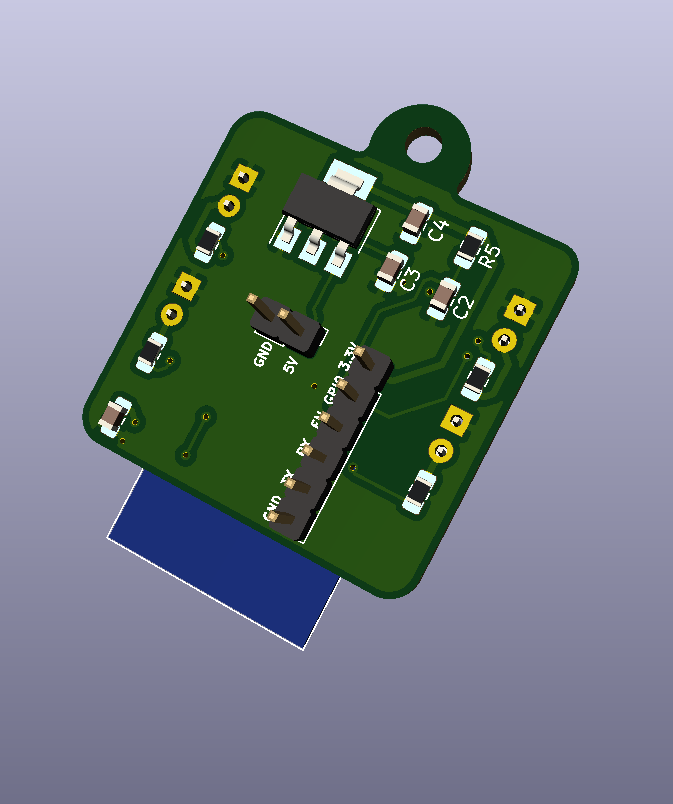
\includegraphics[scale=0.4]{../emiter_2.PNG}
    \subsection{Imágenes reales}

\section{Bibliografía}
https://www.bluetooth.com/
\end{document}